% Draft for IEEE Open Journal of the Communications Society (OJ-COMS).
% Formatted with IEEEtran; move the text into the official OJ-COMS template
% from the IEEE Author Center before submission.
\documentclass[journal]{IEEEtran}

\usepackage{amsmath,amssymb,amsthm}
\usepackage{graphicx}
\usepackage{booktabs}
\usepackage{array}
\usepackage{cite}
\usepackage{url}

\theoremstyle{plain}
\newtheorem{result}{Result}

\newcommand{\E}{\mathbb{E}}
\newcommand{\ns}{\,\mathrm{ns}}
\newcommand{\ps}{\,\mathrm{ps}}

\begin{document}

\title{Recursive Clock Tracking for Photon-Counting Quantum Key Distribution: Kalman Synchronization, Error and Lock-Loss Analysis, and Finite-Key Performance}

\author{\IEEEauthorblockN{Author names to be completed}
\IEEEauthorblockA{Affiliations to be completed}%
\thanks{Manuscript draft. Numerical results are simulation based.}}

\maketitle

\begin{abstract}
Single-photon detectors in quantum key distribution (QKD) are gated for about 2~ns, so the receiver must know the arrival time of every photon to a small fraction of a nanosecond. Recent work recovers the clock directly from the quantum signal, either by fitting batches of detection times or by comparing histograms of consecutive acquisitions, but these estimators discard what they have learned at every correction and degrade when detections are rare. We treat clock recovery for photon-counting QKD as a state-estimation problem with sparse, randomly timed, outlier-contaminated measurements. We propose a Kalman tracker of the timing offset and drift that is updated after every detection, rejects dark counts with an innovation gate, and runs either on a small share of pilot pulses or directly on the ordinary key detections without any extra photon. We derive the steady-state timing error, the probability of losing lock, and a minimum-pilot design rule, and check them against Monte Carlo simulation. In a decoy-state BB84 link with composable finite-key bounds, simulated with $10^{11}$--$3\times10^{14}$ pulses per figure, Kalman tracking on key detections lowers the RMS gate error by a factor of 3--5 relative to a histogram method in the style of Millet \emph{et al.} and by more than 10 relative to batch re-synchronization, from 25 to 125~km, and it is the only method that still retains a substantial fraction of the ideal key rate at 125~km, although the absolute rate there is small. A classical timing reference matches the tracker only if its residual error is below about 0.2~ns; in addition, a delay of such a reference can leak up to 0.45~bit per sifted bit under detector mismatch, which in-band synchronization absorbs. All results are from simulation, and the assumptions are stated.
\end{abstract}

\begin{IEEEkeywords}
Quantum key distribution, clock synchronization, Kalman filter, finite-key analysis, decoy states, time-shift attack.
\end{IEEEkeywords}

\section{Introduction}
\IEEEPARstart{Q}{uantum} key distribution (QKD) lets two parties establish a secret key whose security rests on physical law, and the BB84 protocol \cite{bb84} with weak coherent pulses and decoy states \cite{hwang2003,lo2005,lim2014} is the basis of most deployed systems. A practical receiver opens a detector gate of a couple of nanoseconds around each expected arrival. If the receiver clock is offset by a few nanoseconds, drifts by parts per million, or wanders, the photons fall outside the gate, the key rate collapses, and the share of dark counts in the detections rises. Clock synchronization is therefore as much a part of the link budget as fibre loss.

The conventional solution is a separate timing channel, such as a bright synchronization laser or a White Rabbit link \cite{whiterabbit2011}. It needs extra hardware and fibre, and it adds an attack surface (Sec.~\ref{sec:security}). A growing body of work instead recovers the clock from the quantum signal itself. Qubit4Sync \cite{calderaro2020} correlates the detection times with a known qubit sequence, Cochran and Gauthier \cite{cochran2021} use Bayesian batch estimation, and further variants and field trials have been reported \cite{krause2025,chen2023,guan2025,spiess2023,tiefenthaler2026}. The most recent proposal, by Millet \emph{et al.} \cite{millet2026}, estimates drift and offset from the circular means of two consecutive timing histograms of the key detections, needs no extra photons, and was validated on commercial hardware. All of these estimators work in batches: a correction is computed from a window of detections and applied, and the next window starts afresh. They cannot weigh old against new information, and the estimate is frozen between corrections, which is costly when detections are rare (a few pilot detections per millisecond at 100~km) or the oscillator wanders.

Kalman filtering is a standard tool for exactly this situation. In QKD it has been applied to track the reference phase and polarization of continuous-variable systems from bright pilot signals \cite{wang2019,huang2020,chin2021,kasthuri2024,ma2022}, and in classical networks it underlies clock servos for IEEE~1588 and wireless sensor networks \cite{hamilton2008,giorgi2011,giorgi2013}. To our knowledge it has not been applied to clock tracking from sparse single-photon detections in photon-counting QKD, where the measurements are Poisson-timed clicks, a fraction of which are dark-count outliers, and where a lost lock is catastrophic. That is the gap addressed here.

The contributions of this paper are:
\begin{enumerate}
\item A two-stage clock estimator for photon-counting QKD: drift-search acquisition on a short preamble, followed by a Kalman tracker of offset and drift that is updated after every detection and rejects dark counts with an innovation gate. It runs on pilot pulses or, with no extra photons, on the key detections (Sec.~\ref{sec:methods}).
\item An analytical model of the tracker: the steady-state timing error, the probability of losing lock, and a minimum pilot overhead as a function of distance and oscillator quality, validated against simulation (Sec.~\ref{sec:analysis}).
\item A benchmark of eight synchronization strategies under composable decoy-state finite-key bounds, in which the two published estimator families are tuned to their best settings (Sec.~\ref{sec:results}).
\item A timing-layer security analysis: the leakage caused by delaying a classical reference, the absorption of such a delay by in-band synchronization, a variance test for random time shifts, and a bound on the leakage of synchronizing on key detections (Sec.~\ref{sec:security}).
\end{enumerate}

\section{System Model}
\label{sec:model}
Figure~\ref{fig:system} shows the link. Table~\ref{tab:params} lists the default parameters, which are used throughout unless stated.

\begin{figure*}[t]
\centering
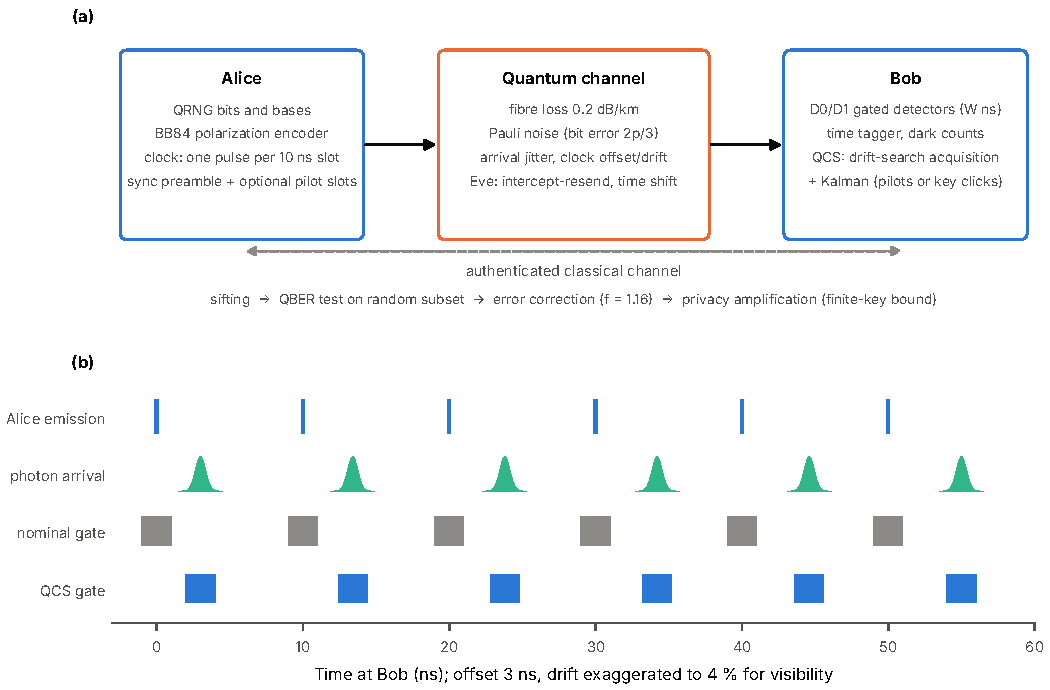
\includegraphics[width=\textwidth]{figures/fig01_system_model.pdf}
\caption{System model. (a) Alice, the fibre channel and Bob, with the synchronization loop and the classical post-processing chain. (b) Timing diagram: photon arrivals are shifted by clock offset and drift, so the nominal gates miss them, while the synchronized gates catch them.}
\label{fig:system}
\end{figure*}

\begin{table}[t]
\caption{Default simulation parameters.}
\label{tab:params}
\centering
\small
\begin{tabular}{@{}ll@{}}
\toprule
Parameter & Value \\
\midrule
Slot period $T$ & 10~ns \\
Fibre loss, detector efficiency & 0.2~dB/km, 0.6 \\
Dark counts, gate width $W$ & $10^4$~Hz per detector, 2~ns \\
Arrival jitter $\sigma$ & 0.35~ns (Gaussian) \\
Initial offset, drift & 4~ns, 20~ppm \\
Oscillator wander $w$ & 0.01 (stable), 0.2 (poor) ppm/$\sqrt{\mathrm{ms}}$ \\
Intensities $\mu_1,\mu_2,\mu_3$ & 0.5, 0.2, 0.0002 \\
Intensity probabilities, $p_Z$ & 0.6, 0.2, 0.2; 0.8 \\
Channel bit error & 2\% (Pauli $p=0.03$) \\
$f_{\mathrm{EC}}$, $\varepsilon_{\mathrm{sec}}$, $\varepsilon_{\mathrm{cor}}$ & 1.16, $10^{-10}$, $10^{-15}$ \\
Key block, timing segment & $10^{10}$ slots (100~s), $10^{8}$ slots (1~s) \\
Pilot share, classical residual & 1\%, 0.5~ns (rms) \\
Preamble & 64 expected detections, spacing 5 slots \\
\bottomrule
\end{tabular}
\end{table}

\subsection{Source, channel and detection}
Alice emits one pulse per slot with intensity $\mu_k$ chosen with probability $p_k$ and encodes it in the $Z$ basis with probability $p_Z$ and the $X$ basis otherwise; Bob chooses his basis in the same way. Let $T_{\mathrm{ch}}=10^{-\alpha L/10}$ be the fibre transmittance for loss $\alpha$ and length $L$, and $\eta=\eta_d T_{\mathrm{ch}}$ the total efficiency with detector efficiency $\eta_d$. If the photon falls inside the gate with probability $c$ (the timing capture, below) and the dark-click probability per gate is $p_d=1-e^{-2R_d W}$ for dark rate $R_d$ and two detectors, a slot with intensity $\mu$ yields a click with probability and an error with probability
\begin{align}
p_{\mathrm{ph}}(\mu) &= 1-e^{-\eta c\mu}, \qquad p_{\mathrm{click}}(\mu)=p_{\mathrm{ph}}+(1-p_{\mathrm{ph}})\,p_d, \label{eq:click}\\
p_{\mathrm{err}}(\mu) &= \big[p_{\mathrm{ph}}(1-p_d)\,e_{\mathrm{sig}}+\tfrac12 p_d\big]/p_{\mathrm{click}}(\mu). \label{eq:err}
\end{align}
Here $e_{\mathrm{sig}}$ is the bit error of a genuine click, combining channel noise $e_{\mathrm{ch}}$ and an intercept-resend fraction $f$ of a spy as $e_{\mathrm{ch}}(1-f/4)+(f/4)(1-e_{\mathrm{ch}})$. Poor timing lowers $c$, which reduces the genuine clicks while leaving the dark clicks unchanged and therefore raises the error.

\subsection{Timing layer}
Relative to Bob's nominal gate schedule, a photon sent at time $t$ arrives with the timing error
\begin{equation}
e(t)=e_0+\nu_0 t+w(t)+\varepsilon, \qquad \varepsilon\sim\mathcal N(0,\sigma^2),
\label{eq:error}
\end{equation}
where $e_0$ is the initial offset, $\nu_0$ the fractional frequency offset (drift), $w(t)$ the integrated random-walk frequency noise of Bob's oscillator, and $\varepsilon$ the arrival jitter. The random walk is characterized by a diffusion constant $q=(w\cdot10^{-6})^2/10^{6}~\mathrm{ns}^{-1}$ for a wander $w$ in ppm$/\sqrt{\mathrm{ms}}$. Bob opens a gate of width $W$ at his estimate $\hat e(t)$. With gate error $d(t)=e(t)-\varepsilon-\hat e(t)$, the capture probability is
\begin{equation}
c(d)=\Phi\!\left(\frac{W/2-d}{\sigma}\right)-\Phi\!\left(\frac{-W/2-d}{\sigma}\right),
\label{eq:capture}
\end{equation}
with $\Phi$ the standard normal distribution function. For $W=2$~ns and $\sigma=0.35$~ns, a perfect clock gives $c=99.57\%$, a gate error of 0.5~ns gives 92.4\%, 1~ns gives 50\%, and 2~ns gives 0.2\%. We average $c$ over the key part of the timing segment and call this the timing capture. Synchronization determines $\hat e(t)$; its quality is measured by the RMS gate error and the capture.

\subsection{Finite-key rate}
We use the decoy-state finite-key bound of Lim \emph{et al.} \cite{lim2014} with three intensities. From the $Z$ detections $n_Z$ and errors $m_Z$ and the $X$ detections $n_X$ and errors $m_X$ at each intensity, widened by Hoeffding terms $\delta=\sqrt{(n/2)\ln(21/\varepsilon_{\mathrm{sec}})}$, one bounds the number $s_0$ of vacuum and $s_1$ of single-photon $Z$ detections and the single-photon phase error $\varphi$. The secret key length is
\begin{equation}
\ell = s_0 + s_1\big[1-h(\varphi)\big]-\lambda_{\mathrm{EC}}-6\log_2\frac{21}{\varepsilon_{\mathrm{sec}}}-\log_2\frac{2}{\varepsilon_{\mathrm{cor}}},
\label{eq:key}
\end{equation}
with $h$ the binary entropy, $\lambda_{\mathrm{EC}}=f_{\mathrm{EC}}\,n_Z\,h(e_Z)$ the error-correction leakage, and a block is rejected if $\ell\le0$. The key rate is $\ell$ divided by the number of slots of the key block, in bits per slot (multiply by the pulse rate for bits per second). Slots spent on preamble and pilots are removed from the key slots, so synchronization is paid for in the key rate. The asymptotic rate, computed from the same counts without the margins, and the PLOB bound \cite{plob2017} serve as references.

\subsection{Two time scales}
Timing is simulated pulse by pulse over a segment of $10^{8}$ slots (1~s), including the preamble, the pilots or key detections, the dark counts and the estimator. The resulting timing capture is then applied to the whole key block of $10^{10}$ slots (100~s), whose detection counts are drawn exactly from binomial and multinomial distributions. This assumes that the synchronization is statistically stationary after the first second, which holds for a locked tracker; it is listed among the limitations in Sec.~\ref{sec:discussion}.

\section{Synchronization Strategies}
\label{sec:methods}
All strategies return an estimate $\hat e(t)$. We compare eight: no synchronization ($\hat e=0$); a classical reference (a constant residual drawn from $\mathcal N(0,0.5^2)$~ns per block, with no photons used); preamble-only QCS (stage~1 below, extrapolated); batch re-synchronization; histogram re-synchronization; Kalman tracking on pilots; Kalman tracking on key detections; and perfect synchronization ($\hat e=e$).

\subsection{Acquisition (stage 1, common to all QCS methods)}
Alice sends a preamble of one sync pulse every 5 slots (50~ns) until about 64 detections are expected. Bob time-tags every click. Each tag is known only modulo the preamble spacing, since Bob does not know which pulse produced it, and dark counts are uniform over the spacing. For every candidate drift $\nu$ on a grid over $\pm100$~ppm, the tags are de-rotated by $\nu t$, wrapped, and histogrammed in bins of width $2\sigma$; the $\nu$ with the tallest peak is selected. Tags within $3\sigma$ of the peak are unwrapped and a least-squares line gives the offset, the drift and their covariance (a $2\times2$ matrix) at the last tag. The accuracy of this stage is compared with the Cram\'er--Rao bound in Sec.~\ref{sec:analysis}. Preamble-only QCS extrapolates this line for the whole block; with a drift known to $\sim10^{-7}$ the gate is lost within milliseconds.

\subsection{Batch re-synchronization (prior art)}
Representative of Qubit4Sync-type methods \cite{calderaro2020,cochran2021}, and run on pilot pulses (one per 100 slots). Bob predicts each pilot click from the current line, records the residual of the clicks that fall within $\pm T/2$, and after 32 clicks repeats the drift-search fit of stage~1 on the residuals ($\pm100$~ppm), adds the result to the line and holds it until the next batch is complete.

\subsection{Histogram re-synchronization (after Millet et al.)}
Following \cite{millet2026}, which uses the key detections and no pilots, the residuals of the detection times are folded onto the slot period $T$ and mapped to phases $\theta=2\pi r/T$. Two consecutive histograms of duration $T_{\mathrm{int}}$ give circular means $m_1=\E[e^{i\theta}]$ and $m_2$. The drift and offset corrections are
\begin{equation}
\hat\nu=\frac{T}{2\pi T_{\mathrm{int}}}\arg(m_2\bar m_1),\qquad
\hat\tau=\frac{T}{2\pi}\arg(m_2)+\hat\nu\frac{T_{\mathrm{int}}}{2},
\end{equation}
applied once per pair. The windows start at about 10 detections and grow by a factor of 4 after every three corrections up to a maximum duration, as in the paper's start-up schedule. Because the best maximum duration depends on distance and oscillator quality, we simulate 100~$\mu$s, 300~$\mu$s, 1~ms and 3~ms and keep the best at every point (Sec.~\ref{sec:results}). This is our reimplementation from the published description, not the authors' code.

\subsection{Kalman tracking (this work)}
The state is $\mathbf x=[\tau,\nu]^\top$ (timing error and drift) with covariance $\mathbf P$. During a gap $\Delta$ since the last update,
\begin{align}
\mathbf x^- &= \mathbf F\mathbf x,\quad \mathbf F=\begin{bmatrix}1&\Delta\\0&1\end{bmatrix},\\
\mathbf P^- &= \mathbf F\mathbf P\mathbf F^\top+q\begin{bmatrix}\Delta^3/3&\Delta^2/2\\ \Delta^2/2&\Delta\end{bmatrix}, \label{eq:predict}
\end{align}
where the drift performs a random walk of strength $q$ and, with it, the timing error. A detection with time tag $z=\tau+n$, $n\sim\mathcal N(0,r)$, $r=\sigma^2$, produces the innovation $y=z-\tau^-$ with variance $S=P^-_{11}+r$. It is rejected as a dark count if $y^2>\gamma^2 S$ ($\gamma=3$) and otherwise used:
\begin{equation}
\mathbf K=\mathbf P^-\mathbf h^\top/S,\quad
\mathbf x=\mathbf x^-+\mathbf K y,\quad
\mathbf P=(\mathbf I-\mathbf K\mathbf h)\mathbf P^-, \label{eq:update}
\end{equation}
with $\mathbf h=[1,0]$. The initial state and covariance come from acquisition. The state has two elements, so the cost per detection is a few multiplications. It carries its uncertainty from update to update: after a long silence $P^-_{11}$ is large and the next detection is trusted more, while after many detections the gain falls and each detection moves the estimate only a little. The process noise $q$ is set from the oscillator wander (with a floor corresponding to 0.005~ppm$/\sqrt{\mathrm{ms}}$).

\emph{Pilot version.} One sync pulse in every 100 slots (1\% overhead); detections are processed as they arrive, and the pilot listening window is the slot, $\pm T/2$ around the prediction.

\emph{Key-detection version.} The same filter runs on the time tags of the key detections (all intensities), with no pilots. The arrival time of a click does not depend on the bit or the basis in an ideal receiver, so every click carries timing information at no cost in photons (security in Sec.~\ref{sec:security}). To keep the computation tractable at short range, up to $10^{6}$ detections per timing segment are used, and they are processed in groups of at most 25: each click is gated against the group prediction, and the accepted tags are averaged into one measurement at their mean time with variance $r/k$ for $k$ accepted clicks. For a linear drift this equals sequential processing; the group spans a few microseconds. The cap makes the short-range accuracy a conservative figure.

\section{Performance Analysis}
\label{sec:analysis}
\subsection{Steady-state timing error}
Let detections arrive as a Poisson process with mean gap $\Delta$ (for pilots $\Delta=n_pT/p_{\mathrm{sync}}$, with $n_p$ slots per pilot and $p_{\mathrm{sync}}=1-e^{-\eta\mu_1}$; for key detections the mean gap between processed clicks). Iterating (\ref{eq:predict})--(\ref{eq:update}) with a fixed gap $\Delta$ converges to a covariance $\mathbf P_\infty$ just after an update (the discrete algebraic Riccati solution). Between updates the error variance at age $t$ is
\begin{equation}
V(t)=P_{11}+2tP_{12}+t^2P_{22}+\tfrac13 q t^3.
\end{equation}
The age of a random instant is exponentially distributed with mean $\Delta$, because the arrivals are memoryless.

\begin{result}[Mean-square gate error]
\label{res:ms}
Using $\int_0^\infty t^n e^{-t/\Delta}\Delta^{-1}\mathrm{d}t=n!\,\Delta^n$,
\begin{equation}
\mathrm{MS}=\E[V]=P_{11}+2P_{12}\Delta+2P_{22}\Delta^2+2q\Delta^3,
\label{eq:ms}
\end{equation}
\end{result}
The RMS gate error is $\sqrt{\mathrm{MS}}$. The terms are: the noise left by the last update, the uncertainty of the drift multiplied by the waiting time, and the wander of the oscillator during the wait. The covariance in (\ref{eq:ms}) is the fixed-gap steady state, which approximates the random gaps.

\subsection{Probability of losing lock}
Two mechanisms are modelled as independent hazards. \emph{Overrun:} if the error leaves the pilot window $\pm h$, $h=T/2$, during a gap $g$, the next pilot is missed and the tracker cannot recover. The miss probability for a gap $g$ is $2[1-\Phi(h/\sqrt{V(g)})]$; averaging over exponential gaps gives $p_{\mathrm{gap}}$ and the rate $\lambda_{\mathrm{over}}=-\ln(1-p_{\mathrm{gap}})/\Delta$. \emph{Dark capture:} a dark click inside the innovation gate is accepted, and is harmful when the prediction is less certain than a single click ($V>r$). With $p_d'$ the dark-click probability per sync slot of period $T_p$ and $a(t)=\min\!\big(1,\gamma\sqrt{V(t)+r}/h\big)$ the fraction of the window accepted by the gate,
\begin{equation}
\lambda_{\mathrm{dark}}=\frac{p_d'}{T_p}\int_0^\infty a(t)\,\mathbf 1[V(t)>r]\,\frac{e^{-t/\Delta}}{\Delta}\,\mathrm dt.
\end{equation}
The probability of losing lock within a segment of duration $T_{\mathrm{seg}}$ is
\begin{equation}
P_{\mathrm{lost}}=1-\exp\!\big[-(\lambda_{\mathrm{over}}+\lambda_{\mathrm{dark}})\,T_{\mathrm{seg}}\big].
\label{eq:lost}
\end{equation}
These formulas are for the pilot tracker. For the key-detection version we give only the error (\ref{eq:ms}); no lock loss was observed in simulation up to 125~km.

\subsection{Design rule}
Solving $P_{\mathrm{lost}}\le1\%$ for $T_{\mathrm{seg}}=1$~s over the pilot spacing $n_p$ gives the smallest pilot share $1/n_p$ that is safe. Table~\ref{tab:design} lists it for three oscillator qualities; the default 1\% suffices up to about 120~km for the stable oscillator, while a poor oscillator at 100~km needs 3.2\%.

\begin{table}[t]
\caption{Minimum pilot share (\% of slots) for $P_{\mathrm{lost}}\le1\%$ per second.}
\label{tab:design}
\centering
\small
\begin{tabular}{@{}lccc@{}}
\toprule
Distance & $w=0.01$ & $w=0.05$ & $w=0.2$ \\
\midrule
50 km & 0.026 & 0.09 & 0.27 \\
75 km & 0.10 & 0.34 & 0.93 \\
100 km & 0.37 & 1.2 & 3.2 \\
125 km & 1.3 & 4.2 & 11 \\
150 km & 4.5 & 14 & 50 \\
\bottomrule
\end{tabular}
\end{table}

\subsection{Accuracy of acquisition}
For a line fitted to $n$ equally spaced measurements of noise $\sigma$, the Cram\'er--Rao bound \cite{kay1993} on the standard deviation of the fitted value at the last point is
\begin{equation}
\sigma_{\mathrm{CRB}}=\sigma\sqrt{\frac{4n-2}{n(n+1)}}\approx\frac{2\sigma}{\sqrt n}.
\end{equation}
For $\sigma=0.35$~ns and $n=64$ this is 86~ps. Our acquisition (Fig.~\ref{fig:validation}c) reaches 96~ps, 11\% above the bound; at $n=32$ it is 7\% above and at $n=16$ 21\% above. With only 4--8 detections, dark counts occasionally mislead the peak search.

\section{Timing-Layer Security}
\label{sec:security}
\subsection{Detector mismatch and time shifts}
The two detectors of Bob (bit 0 and 1) have gates centred at $c_0=-\delta/2$ and $c_1=+\delta/2$ around the synchronized centre, where $\delta$ is the mismatch \cite{makarov2006}. A photon arriving at relative time $s$ is detected by detector $b$ with efficiency $\eta_b(s)=\Phi\!\big(\tfrac{c_b+W/2-s}{\sigma}\big)-\Phi\!\big(\tfrac{c_b-W/2-s}{\sigma}\big)$. If a spy controls the arrival shift $s$, a click reveals the bit with posterior $\eta_1/(\eta_0+\eta_1)$, and the information is $I(s)=1-h\big(\eta_1/(\eta_0+\eta_1)\big)$ bits per sifted bit, without raising the QBER \cite{qi2007,zhao2008}.

\subsection{Delaying a classical reference, and in-band immunity}
If timing comes from a classical reference, a delay by $s$ of that reference shifts Bob's gates relative to the photons by $s$. In-band synchronization derives timing from the photons, so a uniform delay is estimated as part of $e(t)$ and the relative shift remains zero: $I=0$.

\subsection{Random time shifts and a variance monitor}
If the spy shifts each photon by $\pm s$ at random, the tracker cannot absorb it, but the residual variance grows from $\sigma^2$ to about $\sigma^2+s^2$. For $n$ residuals the sample variance is approximately normal with mean $\sigma^2$ and variance $(\mu_4-\sigma^4)/n$ ($\mu_4$ the fourth moment); the monitor raises an alarm when it exceeds the threshold for a false-alarm rate of $10^{-3}$. The moments are estimated from a large sample of detected residuals.

\subsection{Leakage from synchronizing on key detections}
The time tags and the tracker state remain inside Bob's receiver, and only bases and tested bits are announced, so the tracker adds no public channel. In an ideal receiver the arrival time is independent of the bit. The only coupling is the mismatch: a tracker that pools the tags of both detectors is biased by
\begin{equation}
b=\frac{\delta}{2}\,(p_1-p_0),
\end{equation}
where $p_1-p_0$ is the click imbalance between the detectors, which for random bits is about $1/\sqrt N$ for $N$ detected clicks ($10^{-2}$ for $10^4$ clicks, $10^{-3}$ for $10^6$). For $\delta=0.8$~ns and an imbalance of $10^{-3}$ the bias is 0.4~ps and $I\approx9\times10^{-9}$ bit; even for an extreme imbalance of 5\% the bias is 20~ps and $I\approx2\times10^{-5}$ bit. Delays and random shifts imposed by the spy are handled as above, with the monitor now having up to $10^6$ detections instead of $10^2$--$10^4$ pilot clicks. This is a bounded argument with numbers, not a composable security proof of the whole synchronization layer; active injection of false synchronization clicks is not analysed.

\section{Numerical Results}
\label{sec:results}
\subsection{Setup}
All curves come from the simulator described in Sec.~\ref{sec:model}. Each point is the average (or, for timing errors near lock loss, the median) of 50--1\,000 independent blocks of $10^{8}$--$10^{10}$ slots, so that a point rests on $10^{10}$--$10^{12}$ simulated pulses and a figure on $10^{11}$--$3\times10^{14}$. Error bars are 95\% confidence intervals of the mean, and Wilson intervals for proportions; the median relative half-width is 0.002\% for the QBER, 0.1--0.6\% for key rates and 1.1\% for the timing error of Fig.~\ref{fig:main}. All random numbers derive from fixed seeds, and the code and the data behind every marker are provided with this paper. The sync-phase timing error is the RMS of the gate error over the key part of the 1~s segment. We say a run \emph{loses lock} if more than 1\% of the key time has $|d|>W/2+3\sigma=2.05$~ns.

\begin{figure*}[t]
\centering
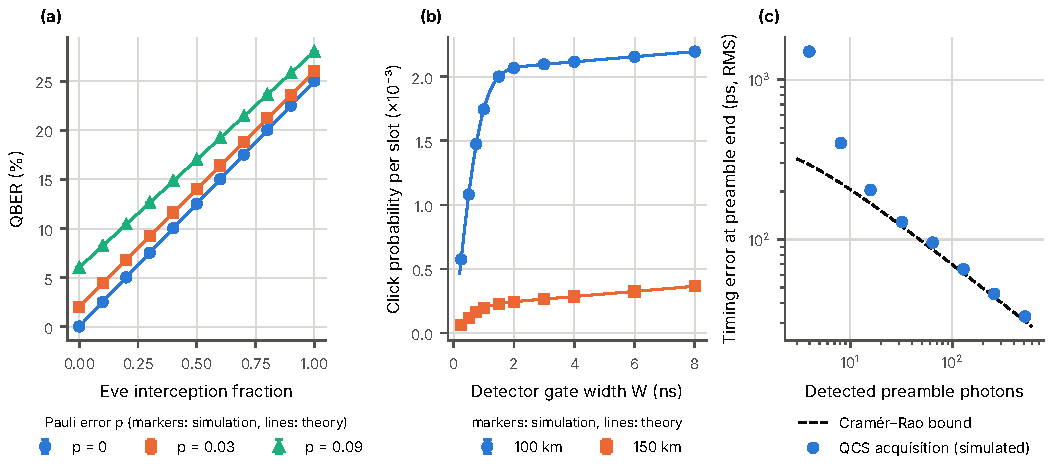
\includegraphics[width=\textwidth]{figures/fig02_model_validation.pdf}
\caption{Model validation. (a) QBER against the spy's interception fraction for three channel noise levels; markers: simulation, lines: closed form. (b) Click probability per slot against gate width at 100 and 150~km; lines: Eq.~(\ref{eq:click}) with Eq.~(\ref{eq:capture}). (c) Timing error after the preamble against the number of detected photons, with the Cram\'er--Rao bound.}
\label{fig:validation}
\end{figure*}

\subsection{Validation}
Figure~\ref{fig:validation} confirms that the simulation reproduces the closed-form QBER, the click statistics, and, in panel (c), that the acquisition error approaches the Cram\'er--Rao bound within 7--11\% for 32--64 detections.

\subsection{Robustness to clock impairments}
Figure~\ref{fig:robust} shows the timing capture at 25~km against initial offset, drift and jitter. Without synchronization the capture is below 1\% except at zero drift. A classical reference with 0.5~ns residual loses 8--12 percentage points (88--92\%), batch re-synchronization keeps 95--97\%, and preamble-only QCS keeps 6--10\% because its extrapolated drift error grows over the block. Kalman tracking on pilots keeps 99.5\% across 0--20~ns offset and 0--200~ppm drift, within 0.05\% of perfect synchronization. At large jitter all methods converge to the limit set by $W/\sigma$.

\begin{figure*}[t]
\centering
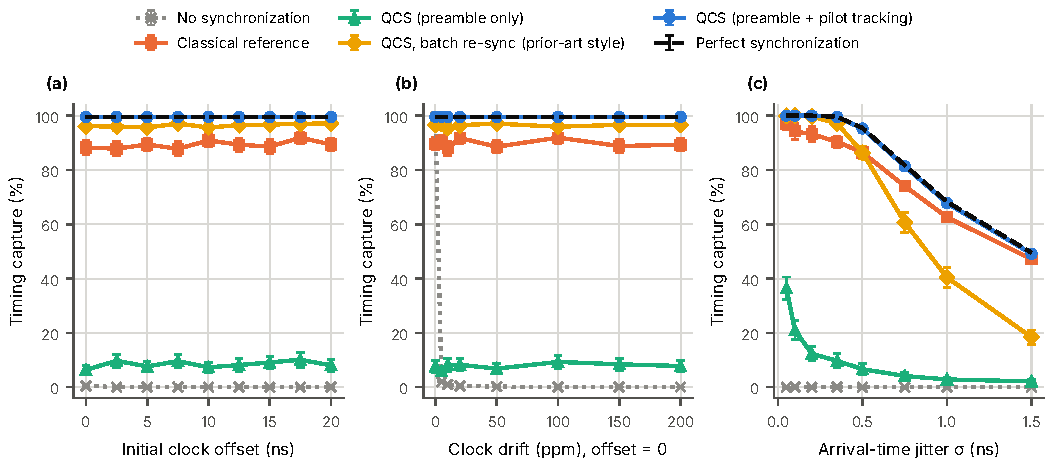
\includegraphics[width=\textwidth]{figures/fig05_timing_impairments.pdf}
\caption{Timing capture at 25~km against (a) initial offset, (b) drift and (c) jitter for no synchronization, classical reference, preamble-only QCS, batch re-synchronization, Kalman tracking on pilots, and perfect synchronization.}
\label{fig:robust}
\end{figure*}

\subsection{Kalman tracking versus published estimators}
Figure~\ref{fig:main} compares the four QCS estimators of Sec.~\ref{sec:methods} for a stable and a poor oscillator, and Table~\ref{tab:main} summarizes it. On the same detections, Kalman tracking on key clicks has a 3--5 times lower RMS gate error than the tuned histogram method (13--39~ps against 40--201~ps for the stable oscillator from 25 to 125~km, 28--84~ps against 81--420~ps for the poor one) and more than 10 times lower than batch re-synchronization (244--818~ps, stable oscillator). It does not lose lock up to 125~km in either case (8\% of the runs lose lock at 150~km with the poor oscillator). Kalman tracking on pilots is 3--10 times more accurate than batch re-synchronization on the same pilots from 10 to 100~km. The batch method loses lock at 125~km with the stable oscillator and from 75~km with the poor one; with the poor oscillator Kalman tracking on pilots holds up to 75~km, keeps 71\% of the ideal key at 100~km, and fails at 125~km. With key detections the tracker is updated every 1--50~$\mu$s instead of every 11~$\mu$s--3.3~ms, which explains its advantage over the pilot version.

\begin{figure*}[t]
\centering
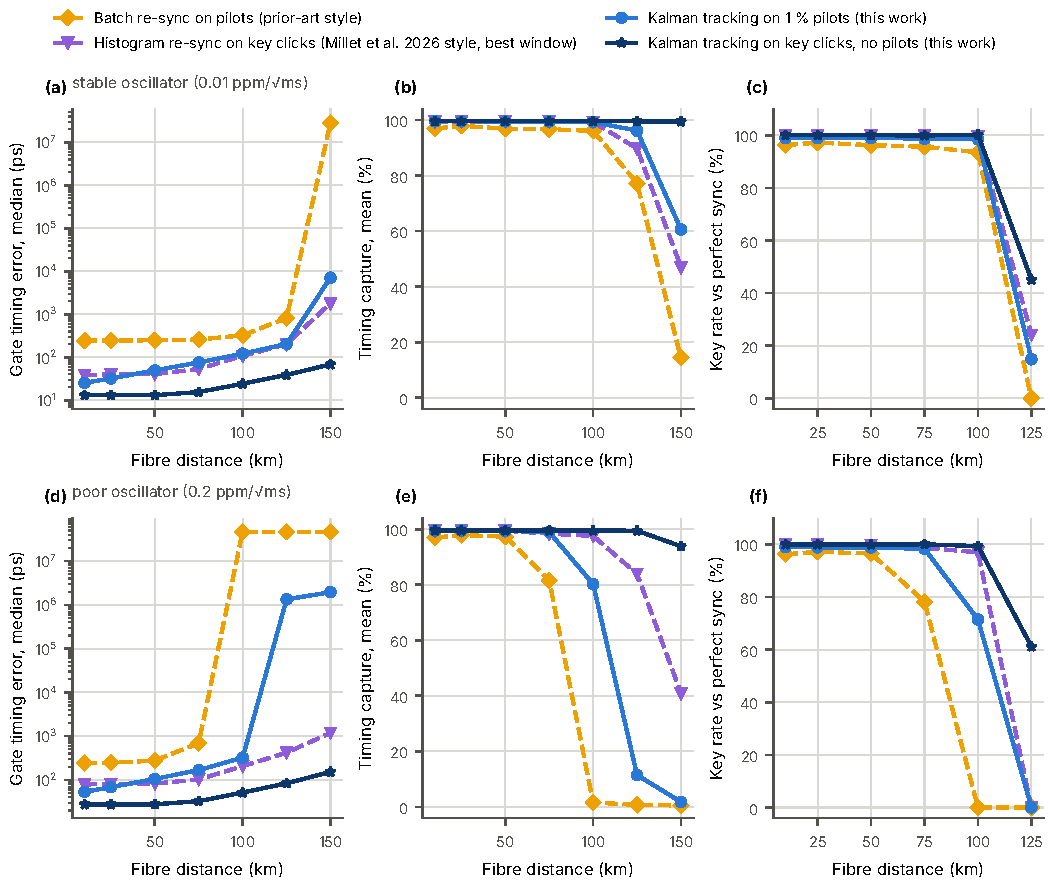
\includegraphics[width=\textwidth]{figures/fig14_kalman_vs_batch.pdf}
\caption{Kalman tracking versus published-style estimators for a stable (top) and a poor (bottom) oscillator: (a, d) median RMS gate error, (b, e) timing capture, (c, f) key rate relative to perfect synchronization. Histogram re-synchronization is tuned to its best duration at every point.}
\label{fig:main}
\end{figure*}

\begin{table}[t]
\caption{Median RMS gate error (ps) and key rate relative to perfect synchronization. ``Lost'': most runs lose lock. Stable / poor oscillator.}
\label{tab:main}
\centering
\small
\setlength{\tabcolsep}{3.5pt}
\begin{tabular}{@{}lcccc@{}}
\toprule
Method & 25~km & 100~km & 125~km & Key at 100 / 125~km \\
\midrule
\multicolumn{5}{@{}l}{\emph{Stable oscillator}}\\
Batch (pilots) & 244 & 323 & 818 & 94\% / 0\% \\
Histogram (key clicks) & 40 & 108 & 201 & 99.5\% / 24\% \\
Kalman (pilots) & 32 & 121 & 204 & 98.5\% / 15\% \\
Kalman (key clicks) & \textbf{13} & \textbf{24} & \textbf{39} & \textbf{100\%} / \textbf{45\%} \\
\midrule
\multicolumn{5}{@{}l}{\emph{Poor oscillator}}\\
Batch (pilots) & 247 & lost & lost & 0\% / 0\% \\
Histogram (key clicks) & 81 & 206 & 420 & 97\% / 0\% \\
Kalman (pilots) & 68 & 323 & lost & 71\% / 0\% \\
Kalman (key clicks) & \textbf{28} & \textbf{51} & \textbf{84} & \textbf{99\%} / \textbf{61\%} \\
\bottomrule
\end{tabular}
\end{table}

\subsection{Key rate against distance}
Figure~\ref{fig:distance} shows the finite-key rate against distance. All methods coincide on the logarithmic scale up to 75~km; the differences are in the relative gap to perfect synchronization (finite key). At 100~km the key rate relative to perfect synchronization is 99.9\% for Kalman on key clicks, 98.0\% for Kalman on pilots, 96.4\% for the tuned histogram method, 93.3\% for batch re-synchronization and 87.8\% for the classical reference; the mean QBER of the histogram method is 4.3\% against 2.9\% for the others, because it includes the 3\% of its runs that lose lock. Kalman tracking on key clicks exceeds the classical reference by 7.5\% at 25~km, 12\% at 50~km, 15\% at 75~km and 14\% at 100~km. At 125~km only the Kalman variants give any key; the rate there is a few hundred bits per block, so the percentages are noisy (58\% of perfect here, 45\% in Fig.~\ref{fig:main}), and nothing is extractable at 150~km with blocks of $10^{10}$ slots. The infinite-key limit for this setup ends at 143~km. Preamble-only QCS gives essentially no key at any distance.

\begin{figure}[t]
\centering
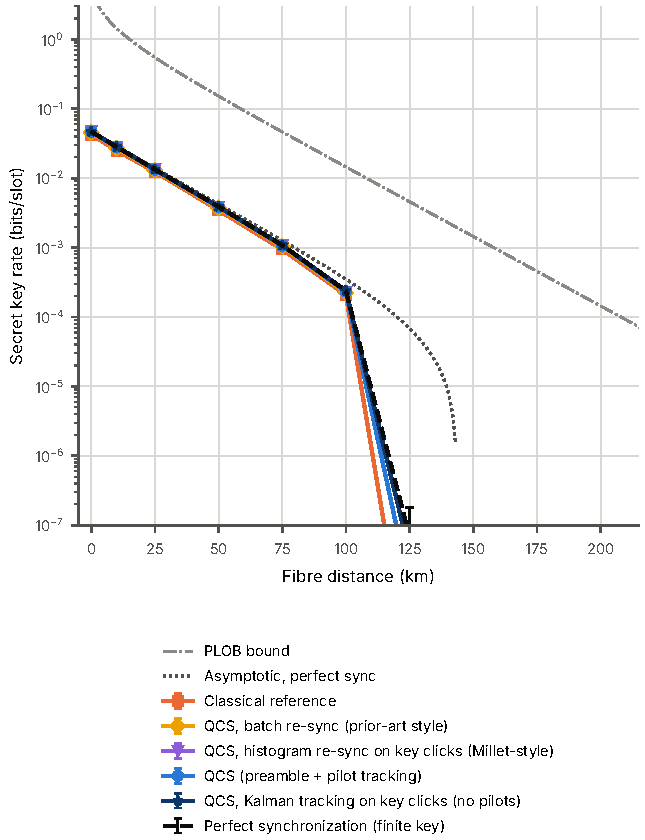
\includegraphics[width=0.92\columnwidth]{figures/fig08_distance.pdf}
\caption{Finite-key secret key rate against distance for the classical reference, batch, histogram (tuned) and Kalman methods, and perfect synchronization, with the asymptotic perfect-synchronization rate and the PLOB bound.}
\label{fig:distance}
\end{figure}

\subsection{Finite-size behaviour}
Figure~\ref{fig:finite} shows the key rate against the key block size from $10^{8}$ to $10^{11}$ slots. At 25~km, Kalman tracking on pilots stays within 1--2\% of perfect synchronization for every size, and the classical reference is 9--16\% lower. At 100~km no key is possible below $3\times10^{9}$ slots, and above it Kalman tracking is within 3\% of perfect synchronization. Both approach the asymptotic limit slowly, which is why the composable bound matters for the comparison.

\begin{figure}[t]
\centering
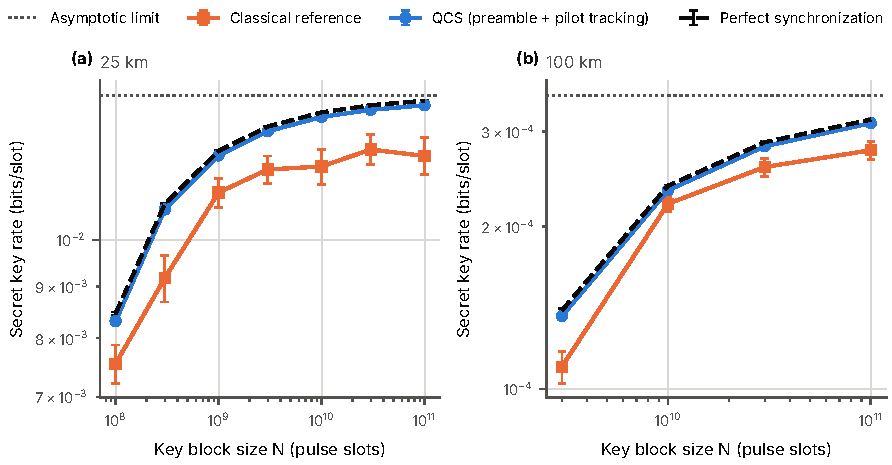
\includegraphics[width=\columnwidth]{figures/fig11_finite_key.pdf}
\caption{Secret key rate against key block size at (a) 25~km and (b) 100~km for the classical reference, Kalman tracking on pilots and perfect synchronization; dotted: asymptotic limit.}
\label{fig:finite}
\end{figure}

\subsection{Theory against simulation}
Figure~\ref{fig:theory} compares (\ref{eq:ms}) and (\ref{eq:lost}) with the simulation. The mean-square error formula reproduces the simulated RMS error for the pilot tracker to within a few percent where the tracker is locked (31.7 against 32.1~ps at 25~km and 117 against 121~ps at 100~km for the stable oscillator; 67 against 68~ps and 286 against 323~ps for the poor one), and for the key-detection tracker, with $\Delta$ replaced by the mean gap between processed clicks, within 1--4\% up to 100~km and 8--9\% at 125~km; at 150~km the simulation is 23--27\% above the theory. The lock-loss formula places the 50\% point at 132~km (stable) and 90~km (poor); the simulation shows 3\% of runs lost at 125~km and 76\% at 150~km (stable), and 41\% at 100~km and 100\% at 125~km (poor), so the boundary is predicted to within one step of the 25~km grid.

\begin{figure*}[t]
\centering
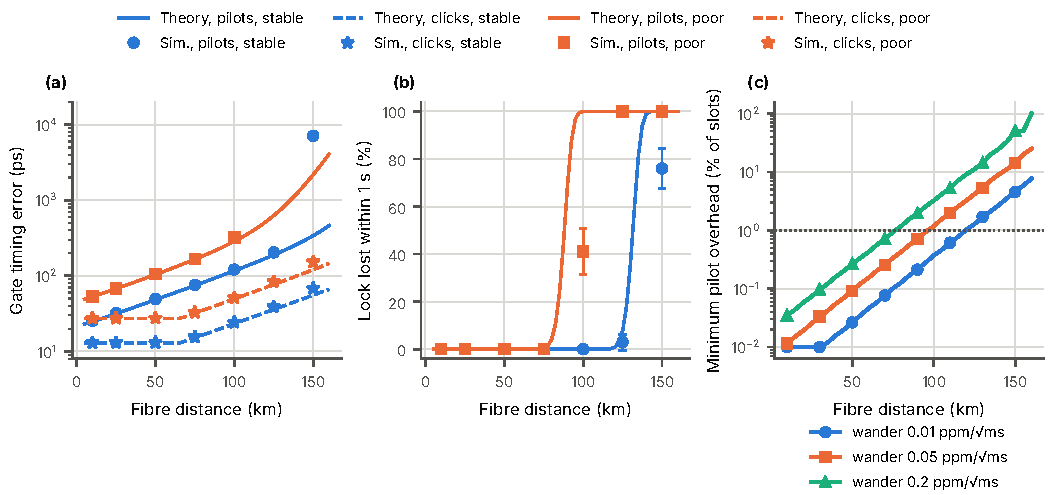
\includegraphics[width=\textwidth]{figures/fig15_tracking_theory.pdf}
\caption{Analytical model against simulation. (a) RMS gate error for pilots (solid) and key clicks (dashed); (b) probability of losing lock within 1~s for the pilot tracker; (c) minimum pilot share against distance for three oscillator qualities.}
\label{fig:theory}
\end{figure*}

\subsection{Fairness checks}
Figure~\ref{fig:fair} tests whether the advantage depends on a poorly tuned baseline. (a) For the poor oscillator, the best batch size (64 clicks, 207~ps at 25~km; 16 clicks, 1.3~ns at 100~km) is still 3 and 4 times worse than Kalman tracking on the same pilots (69 and 287~ps). (b) A classical reference with rms residual below about 0.2~ns achieves at least 99\% of the perfect-synchronization key rate and matches in-band tracking; at 0.5~ns it gives 83--88\% and at 1~ns 56--67\%. The benefit of in-band synchronization over a classical link is therefore not accuracy against a high-quality link, but the removal of the separate link and its attack surface. (c) For the histogram method on the same key detections, the best duration (300~$\mu$s: 80~ps at 25~km and 206~ps at 100~km) is still 3 and 4 times worse than Kalman tracking (28 and 51~ps); short windows are too noisy at long range and long windows let the oscillator wander between corrections.

\begin{figure*}[t]
\centering
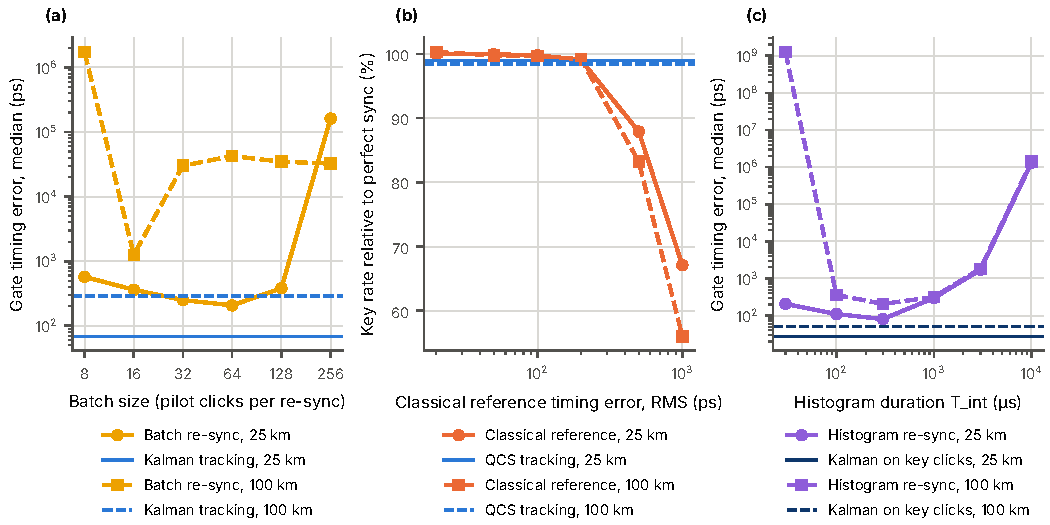
\includegraphics[width=\textwidth]{figures/fig16_fairness.pdf}
\caption{Fairness checks. (a) Batch size of the batch baseline; (b) quality of the classical reference; (c) histogram duration of the histogram baseline, each against the Kalman tracker (horizontal lines).}
\label{fig:fair}
\end{figure*}

\subsection{Timing attacks}
Figure~\ref{fig:attack} shows that delaying a classical reference leaks information without a QBER signature: for 0.8~ns mismatch a 1~ns delay gives $I=0.45$ bit per sifted bit, for 0.4~ns mismatch 0.14 bit, for 0.2~ns mismatch 0.04 bit, while Bob's click rate falls to about half. In-band synchronization absorbs the delay ($I=0$). A random shift of $\pm s$ is flagged with probability above 90\% at a false-alarm rate of $10^{-3}$ for $s=0.325$~ns with 100 detections, 0.175~ns with 1\,000, and 0.10~ns with 10\,000; at these shifts the spy's information is at most $0.0013$ bit (0.4~ns mismatch).

\begin{figure*}[t]
\centering
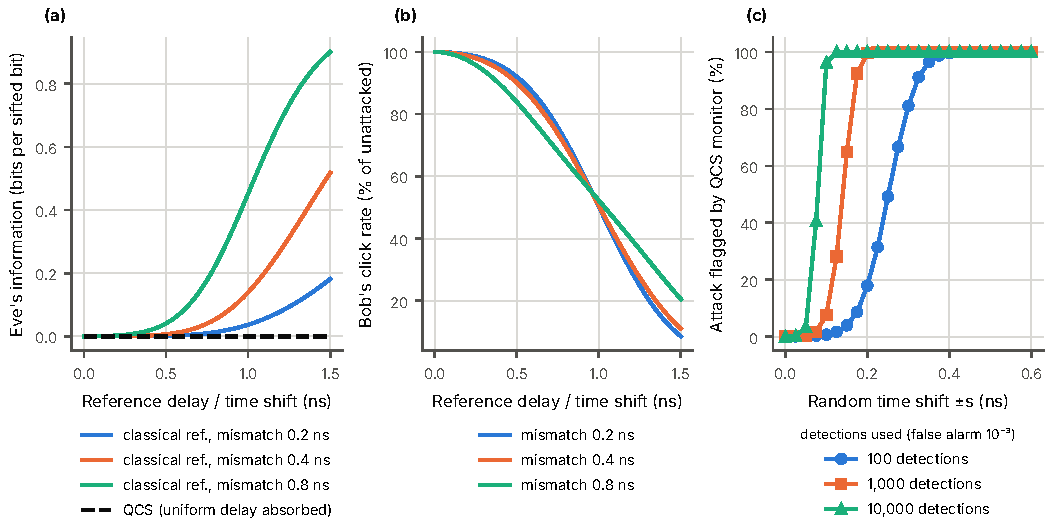
\includegraphics[width=\textwidth]{figures/fig13_timing_attacks.pdf}
\caption{Timing attacks. (a) Information per sifted bit gained by delaying a classical reference for three mismatches; the dashed line is in-band synchronization. (b) Bob's relative click rate under the delay. (c) Detection probability of the variance monitor against a random $\pm s$ shift for 100, 1\,000 and 10\,000 detections.}
\label{fig:attack}
\end{figure*}

\section{Discussion and Limitations}
\label{sec:discussion}
\emph{Practicality.} The tracker has two state variables and one multiplication-level update per detection or group of detections, and it needs only the time tags that the receiver already records. The pilot version needs the sender to insert sync pulses; the key-detection version needs no change at the sender beyond the preamble, which is the reason we regard it as the preferred variant.

\emph{Limitations.} (i) The study is simulation only, while Millet \emph{et al.} validated their method on commercial equipment; their method is our reimplementation from the paper, tuned at every point, and implementation details may differ. (ii) The key block statistics assume stationary synchronization after a 1~s timing simulation. (iii) The lock-loss model is derived for the pilot tracker; the key-detection tracker has a matching error formula but no lock-loss formula, and a lost lock is not recovered in our model. (iv) The process noise $q$ equals the true oscillator wander in our simulations; the sensitivity to a wrong $q$ has not been studied. (v) The security argument of Sec.~\ref{sec:security} is a bounded argument, not a composable proof, and active injection of false clicks is not analysed. (vi) One detector model, a fixed 2~ns gate, and a fibre channel with constant loss were used. (vii) A classical timing link with sub-0.2~ns residual matches the tracker's key rate.

\emph{Future work.} A composable security proof including the synchronization layer; lock-loss theory and re-acquisition for the key-detection tracker; adaptive estimation of $q$; longer timing simulations; and validation on recorded time tags from a QKD system.

\section{Conclusion}
Treating clock recovery in photon-counting QKD as recursive state estimation yields a tracker that updates after every detection, rejects dark counts by innovation gating, and needs no extra photons when run on the key detections. Its timing error and lock-loss probability follow from closed-form expressions that agree with simulation, and the minimum pilot share for a given distance and oscillator is obtained from them. Against published batch and histogram estimators, both tuned to their best settings, it lowers the RMS gate error by factors of 3--5 and more than 10 respectively over 25--125~km, and retains a substantial share of the ideal key rate at 125~km. A classical reference is competitive only below about 0.2~ns of error and can be attacked through detector mismatch, which in-band synchronization absorbs. Experimental validation and a composable security proof for the synchronization layer remain open.

\bibliographystyle{IEEEtran}
\bibliography{references}

\end{document}
